\documentclass[conference]{IEEEtran}
\IEEEoverridecommandlockouts
% AdCONIP 2026 manuscript v2 - built on the IEEE conference template.
% Sections I-III carried over from manuscript.md (v1) as is; abstract and
% Sections IV-VIII rewritten around the matched-floor v5 benchmark of the
% three retained architectures (1-layer EMPC, 2-layer EMPC, SSRTO+3xPI).
% Figures: docs/adconip2026/figs/ (generated by
% scripts/make_adconip_v2_paper_figs.py from
% notebooks/compare_newsim_v5_3model_218h.ipynb data).

\usepackage{cite}
\usepackage{amsmath,amssymb,amsfonts}
\usepackage{graphicx}
\usepackage{textcomp}
\usepackage{xcolor}
\usepackage{booktabs}
\graphicspath{{figs/}}

\begin{document}

\title{A Modular Energy-Minimising Economic MPC for a Single-Stage SAG Grinding Mill: Decoupling Mill Control from Plant-Wide Economics}

\author{\IEEEauthorblockN{Batbold Sangi}
\IEEEauthorblockA{\textit{WA School of Mines} \\
\textit{Curtin University}\\
Perth, Australia \\
batbold.sangi@postgrad.curtin.edu.au}
\and
\IEEEauthorblockN{Agus Saptoro}
\IEEEauthorblockA{\textit{WA School of Mines} \\
\textit{Curtin University}\\
Kalgoorlie, Australia \\
agus.saptoro@curtin.edu.au}
\and
\IEEEauthorblockN{Laurence Dyer}
\IEEEauthorblockA{\textit{WA School of Mines} \\
\textit{Curtin University}\\
Kalgoorlie, Australia \\
laurence.dyer@curtin.edu.au}
\and
\IEEEauthorblockN{Moses O. Tade}
\IEEEauthorblockA{\textit{WA School of Mines} \\
\textit{Curtin University}\\
Perth, Australia \\
m.o.tade@curtin.edu.au}
}

\maketitle

\begin{abstract}
Grinding is the largest energy consumer in a mineral concentrator, so the
choice of economic objective for a semi-autogenous grinding (SAG) mill
controller matters both economically and structurally. This paper compares
the two candidate objectives, profit maximisation and specific-energy
minimisation, across three supervisory architectures on a single-stage
SAG circuit. The architectures are a classical steady-state
RTO over three PI loops (SSRTO+3PI, the industrial reference), a two-layer
economic MPC, and a single-layer economic MPC. All six combinations run on
identical synthetic ore-hardness realisations, an identical product-size
floor, and a common augmented extended Kalman filter, over a 218 h
transient protocol. Such a like-for-like comparison is rarely attempted.
Published architectures each come with their own model, estimator,
constraint set and tuning, so reported differences confound the control
structure with its configuration. Two results stand out. First, at a matched product-size
floor, the specific energy of all architectures and both objectives
clusters within about two percent and follows the ore-hardness
disturbance. A well-chosen optimisation reaches the achievable SEC, and
that achievable SEC is set by the ore hardness and the quality floor,
not by the architecture or the objective. Second, both objectives reach
the same specific energy. Profit optimisation suits the plant-wide
level, and energy minimisation suits the SAG mill level. Energy
minimisation avoids saturated feed and speed, keeps the mill near its
safer lower limits, and supports operator derating. Through the
feed-demand and product-size interface it gives the mill full
modularity, so the SAG controller does not implement the economic
optimisation of the other circuits. Among the architectures, the two-layer EMPC combines
smooth actuation with about a third less computation than the
single-layer EMPC, making it our main candidate. These are early-stage
results on a synthetic plant, obtained within a deliberately contained
simulation scope. Calibration against operating plant data is ongoing.
\end{abstract}

\begin{IEEEkeywords}
economic MPC, real-time optimisation, SAG mill, comminution, specific
energy, plant-wide control
\end{IEEEkeywords}

% =====================================================================
\section{Introduction}
% Section carried over from manuscript v1 as is.

Comminution, the crushing and grinding of ore, is the most energy-intensive
stage of mineral processing. Grinding alone can account for roughly half of
a concentrator's operating cost, and comminution consumes on the order of a
few percent of global electricity. Any systematic reduction in specific
energy consumption (SEC, in kWh per tonne) therefore has both an
economic and an emissions payoff.

A semi-autogenous grinding (SAG) mill is difficult to operate near its
economic optimum because it rarely settles. Ore hardness drifts on an
hour-to-shift timescale, feed-size distribution varies, and liner wear
changes the mill geometry over weeks. This operating reality motivates
economic model predictive control (EMPC). EMPC embeds the process
economics directly in a receding-horizon optimisation. It can therefore
track a moving optimum during transients, rather than waiting for the
plant to settle as a classical real-time optimiser (RTO) must.

The way a supervisory layer decides the economically best operating point
spans a well-known continuum from steady-state RTO (SSRTO) to EMPC, in
which the economic objective is folded into the regulatory controller
itself \cite{matias2022,ellis2017}. Published EMPC studies of
grinding circuits, however, share a design choice that this paper
questions. Their economic objective is a plant-wide net smelter return. It
is a revenue term built from the downstream flotation concentrate mass
flow, its grade and the metal price, minus operating cost
\cite{leroux2019,thivierge2023}. Embedding downstream economics in the
mill controller couples it to a calibrated flotation model, a specific ore
body and a specific market state, so it must be re-identified whenever any
of these change. In the most directly comparable study
\cite{thivierge2023}, the coupled objective was compared only at steady
state.

This paper adopts the opposite separation and makes two contributions.
First, we argue and demonstrate that on a single-stage SAG mill the
revenue term dominates. Electricity cost is a small fraction of revenue,
so a profit-maximising objective has no interior optimum. It drives the
feed rate and mill speed to their upper limits and holds them there. We
therefore propose a modular, mill-specific objective. It minimises
specific energy alone, subject to a product-size floor and a throughput
demand supplied by a higher-level plant-wide economic optimisation
\cite{leroux2019}. This interface decouples the mill controller from
downstream economics and makes it portable across ore bodies and plants.
Second, we report a like-for-like simulation benchmark of the supervisory
continuum. All architectures run on a common reduced-order plant, under a
common transient scenario, with common tuning. They can therefore be
compared fairly on the metric that matters, specific energy. The results
are preliminary and obtained on a synthetic plant. The value here is the
fair comparison and the modular formulation, not a plant-certified
saving.

% =====================================================================
\section{Circuit and Reduced-Order Model}
% Section carried over from manuscript v1 as is.

All controllers act on the same simulated plant. It is a single-stage
closed grinding circuit consisting of a SAG mill, a sump, and a
hydrocyclone (Fig.~\ref{fig:circuit}). The plant dynamics follow the reduced-order,
control-oriented Hulbert model, in the single-stage SAG configuration
analysed and validated by le Roux and co-authors \cite{leroux2013}. The
model lumps the size structure of the charge into rocks, solids and fines
and adds water and ball hold-ups. This gives eight nonlinear states. Five
sit in the mill (water, solids, fines, rocks and balls) and three in the
sump (water, solids and fines).

The manipulated variables (MVs) are the mill feed solids MFS (t/h), the
cyclone feed flow CFF, the sump feed water SFW, and the fractional mill
speed. Mill speed is a manipulated variable rather than a fixed parameter,
giving the optimiser a fourth degree of freedom. The controlled variables (CVs) are the mill charge
filling JT, the sump slurry volume SVOL, and the product particle-size
estimate PSE, the fraction of cyclone-overflow product finer than 75
microns. Mill power draw is a monitored output with a parabolic dependence
on charge and rheology. Grinding is power-driven in this model. Fines
production is proportional to mill power through a specific-energy
parameter. That parameter is exactly the physical lever an
energy-minimising objective trades against product fineness.

The model is credible as a control testbed. It was fitted and validated
on a real single-stage plant \cite{leroux2013}, has been dynamically
validated against industrial step-test data \cite{leroux2022}, and is a
de facto standard testbed in the milling control literature.

Every controller in this study estimates the plant state with the same
augmented extended Kalman filter (EKF). It estimates the eight hold-up
states plus a slowly varying ore-hardness parameter as a ninth state,
following the augmented-EKF observer developed for this model
\cite{leroux2017}. Using one estimator across all controllers
keeps the comparison apples-to-apples, so that only the control law
differs.

\begin{figure}[t]
\centering
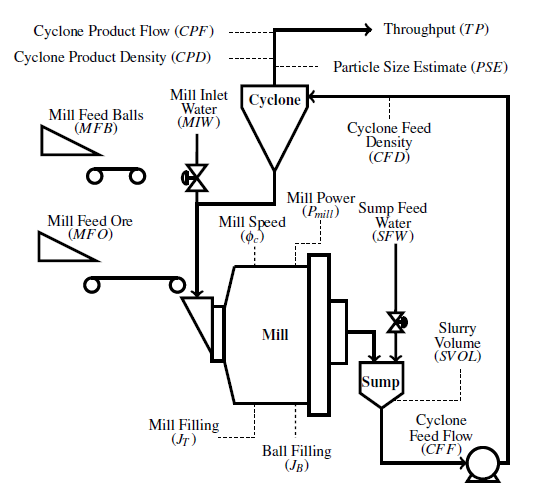
\includegraphics[width=0.82\linewidth]{SAGmill.png}
\caption{Single-stage SAG grinding circuit: mill, sump and hydrocyclone,
with the manipulated variables (feed solids, mill inlet and sump water,
cyclone feed flow, mill speed) and the controlled variables (mill filling,
sump volume, product size).}
\label{fig:circuit}
\end{figure}

% =====================================================================
\section{A Modular Energy-Minimising Cost Function}
% Section carried over from manuscript v1 as is.

\subsection{The plant-wide economic objective}

The economic objective of a grinding mill is not properly defined on the
mill alone. Following the plant-wide framework of le Roux and Craig
\cite{leroux2019}, the comminution circuit's scalar economic objective is
inherited from the larger plant:
\begin{equation}
J_{\mathrm{comm}} = A(\mathrm{PSE})\,\mathrm{TP} - B\,P_{\mathrm{mill}},
\label{eq:jcomm}
\end{equation}
where TP is throughput, $P_{\mathrm{mill}}$ is mill power, $B$ is the
effective energy-plus-media price in dollars per kWh, and $A(\mathrm{PSE})$
is a net return per tonne that folds in the flotation recovery and
concentrate grade, both empirical functions of PSE. This objective has a real
optimum inside the operating range, not on a limit. Feeding more tonnes
makes the grind coarser, and a coarser product returns less per tonne
through recovery and grade. Beyond some point, the extra tonnes are worth
less than the value lost on every tonne. The plant-wide layer maximises
this objective on a slow, event-triggered cadence and hands the
comminution circuit a desired product size and a desired throughput
\cite{leroux2019}. In this study we take $A$ as a constant to simplify
the calculation. The PSE-dependent part of $A$ is a second-order effect
over the narrow PSE band the quality floor allows.

The key observation is that this interface, a product-size floor and a
throughput demand, is exactly what a mill-level controller needs as its
constraints. The plant-wide layer deals with the downstream economics,
which change with prices and markets. The mill controller does not have
to.

\subsection{Mill-level profit maximisation and its side effects}

If the revenue term is instead placed directly in a mill controller, as
$-A\cdot\mathrm{TP} + B\,P_{\mathrm{mill}}$, the objective pursues two
goals at once. It maximises revenue and minimises mill power. The energy
half still disciplines every tonne. Section~VI shows the profit runs match
the energy runs in specific energy. The two goals are not balanced,
though. Revenue exceeds energy cost by about two orders of magnitude. The
stage cost is therefore near-affine in throughput, and its optimum sits on
a constraint boundary. The optimiser raises feed and mill speed until a
limit stops them, and holds them there. Running the mill at maximum speed
continuously, regardless of throughput, is neither good nor common
practice. Liner and media wear grow steeply with speed, and the model
carries no wear cost to push back. Profit at the mill can still be a good
choice, for example when the mill is the plant bottleneck and every extra
tonne has value.

Our simulations confirm this directly (Section~VI). The profit runs park
the feed near its upper bound, the energy runs settle at the demanded
floor, and their specific energies are essentially identical.

\subsection{The modular energy-minimising objective}

We therefore lift the revenue term out of the mill controller entirely.
The plant-wide layer sets the product-size floor and the throughput
demand. The mill controller minimises mill energy for those targets:
\begin{equation}
\min \; B\,P_{\mathrm{mill}}
\quad \text{s.t.}\;\; \mathrm{PSE}\ge \mathrm{PSE}_{\min},\;
\mathrm{MFS}\ge \mathrm{TP}_{\mathrm{dem}},
\label{eq:sec}
\end{equation}
together with the safety envelope on charge, sump volume and power. The
feed settles at the demand floor, so minimising
$P_{\mathrm{mill}}$ is equivalent to minimising
$\mathrm{SEC}=P_{\mathrm{mill}}/\mathrm{MFS}$. SEC itself is the
reported metric, computed as total energy over total tonnes and suitable
for comparison.

One caveat carries over from the affine structure. When the quality floor
is already satisfied, energy cost is nearly flat in feed. With no clear
optimum, the controller swings between its actuator bounds. Move
suppression alone only damps it. The cure is a longer prediction horizon
and keeping the quality constraint binding. The two-layer architecture of
the next section is built to do exactly that.

% =====================================================================
\section{Benchmark Architectures}

We retain three architectures that span the practical range from industrial
practice to fully economic control. All three consume the same augmented
EKF state estimate and face the same constraint set. Each is run twice,
once per economic objective (energy minimisation and profit maximisation).
This gives six 218 h closed-loop runs.

\subsubsection{SSRTO over three PI loops (classical reference)}
This is the popular industrial archetype. A steady-state RTO solves a
parameter-estimation and economic optimisation problem whenever a
steady-state detector declares the plant settled. It hands set-points to
three decentralised PI loops (feed to filling, cyclone feed to sump
volume, sump water to product size). Mill speed is applied directly from
the optimiser. Between steady-state detections the set-points are held.

\subsubsection{Two-layer EMPC (main candidate)}
A slow upper EMPC computes the economic operating point over a long
horizon and publishes a validated set-point-and-input plan. A fast lower
tracking MPC with move suppression executes it (Fig.~\ref{fig:twolayer}).
The economic decision is decoupled from the moment-to-moment actuation,
which removes the single-layer bang-bang failure mode. The expensive
economic problem is also solved far less often. In our 218 h replays the
two-layer used about a third less CPU time than the single-layer EMPC
(13\,336 s versus 19\,682 s), and the SSRTO used two orders of magnitude
less than either (317 s).

\subsubsection{Single-layer EMPC}
The economic objective sits directly in the receding-horizon regulator, so
the economics are re-optimised every 30 s. This is the most
responsive formulation, but the near-affine economic surface makes it
prone to occasional bang-bang actuation when the quality floor is already
satisfied (Section~VI).

Because the three architectures land within about two percent of one
another on every economic metric we measure (Section~VI), secondary
properties decide the ranking. On that basis the two-layer EMPC is our
main candidate (Section~VII).

We also studied basic regulatory control, a tracking single-layer MPC
and a decentralised 3PI system holding fixed set-points with no economic
optimisation layer. We excluded them from the benchmark.
They contain no economic optimisation, so mixing them into the results
would confuse the apples-to-apples comparison between the optimising
architectures.

\begin{figure}[t]
\centering
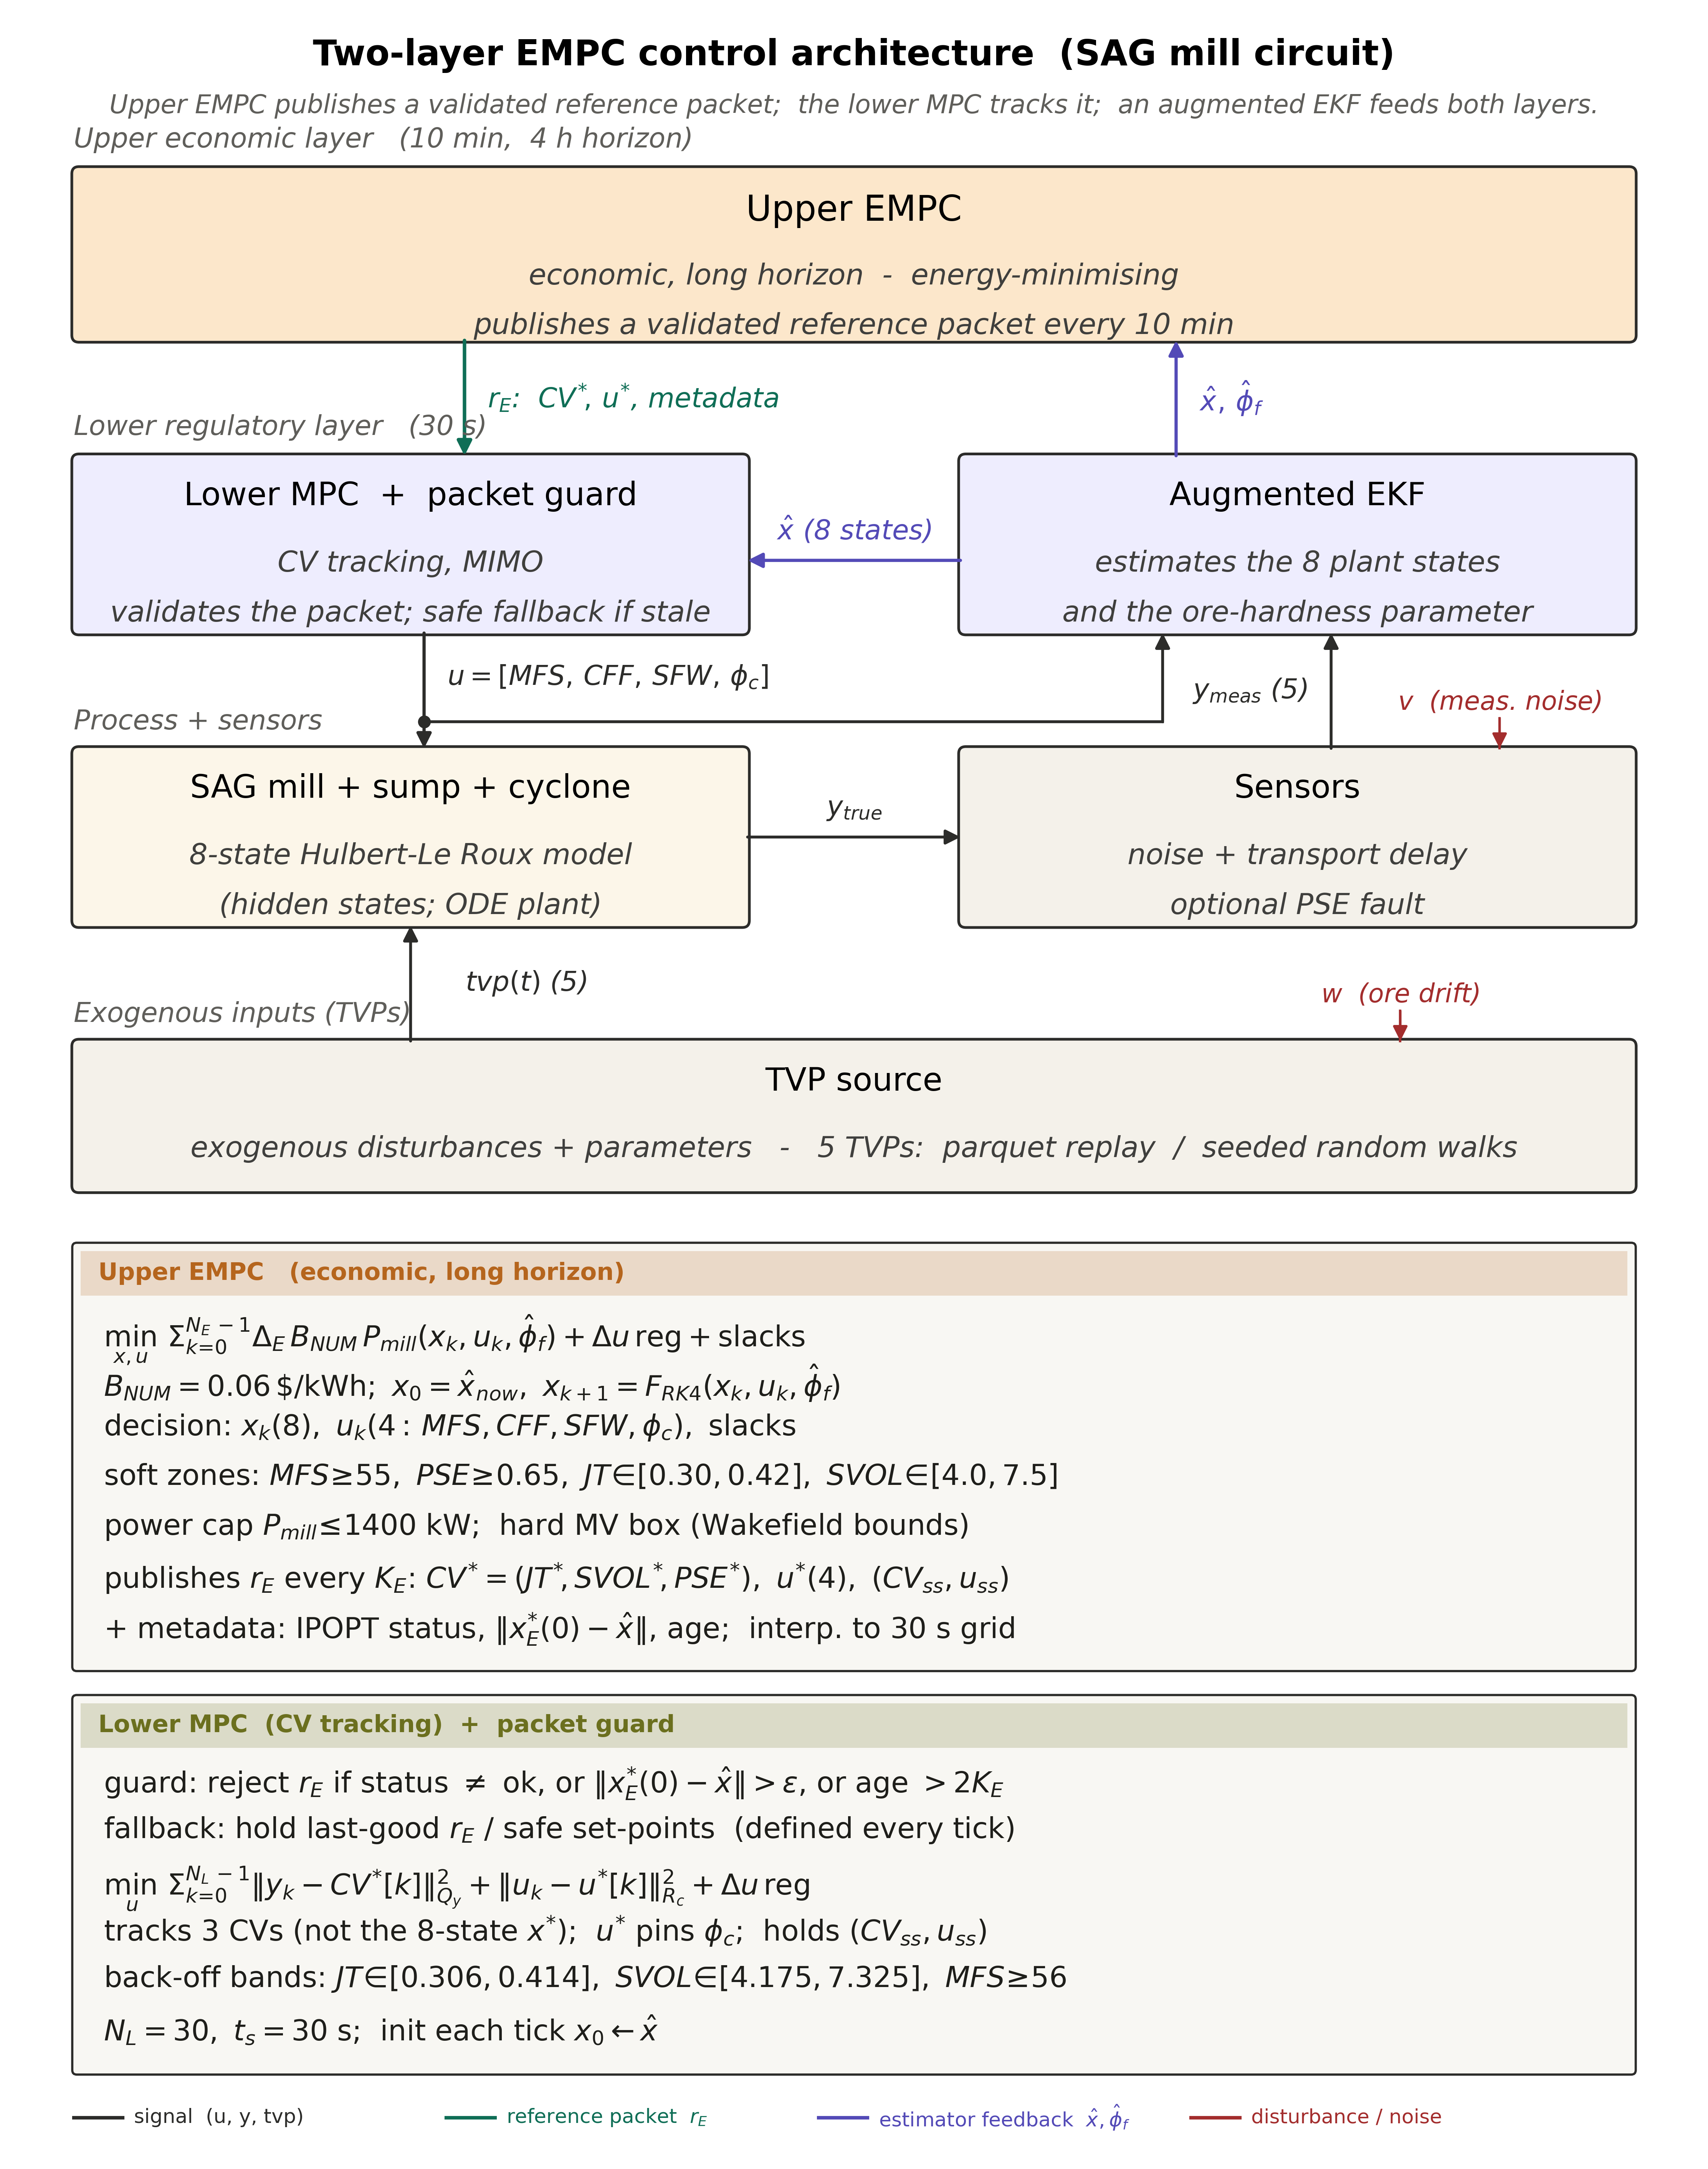
\includegraphics[width=0.72\linewidth]{empc_2layer_v2_milling_circuit.png}
\caption{Two-layer economic MPC architecture. The upper layer minimises
mill energy for the product-size floor and throughput demand inherited from
the plant-wide layer, and publishes a validated set-point-and-input packet;
a guard admits or rejects each packet before the lower tracking MPC and the
augmented EKF close the loop on the plant.}
\label{fig:twolayer}
\end{figure}

% =====================================================================
\section{Benchmark Design}

\textbf{Common plant and scenario.} The plant is integrated with a stiff
solver on a 30 s control interval. Every run sees the same 218 h
three-phase scenario. The first 50 h are a quiescent warm-up. Sensor
noise and bounded ore-hardness disturbances then switch on together. The
noise is a per-channel ladder calibrated to plant instrument noise, from
0.1 to 2 percent of each signal. The ore-hardness parameters move inside
bands of 15 percent ($\alpha_r$) and 10 percent ($\phi_f$) around
nominal. At 75 h the product-size floor steps up by ten percent (0.65 to
0.715). The ore-hardness realisation, shown in the upper panels of
Fig.~\ref{fig:oresec}, drives the rock-fraction parameter $\alpha_r$ and
the feed-size parameter $\phi_f$ through triangle-wave trends with two
extended joint holds. The identical realisation is replayed to every
controller, so differences downstream are attributable to the
architecture and objective alone.

\textbf{Matched constraint set.} All six runs share one operating
envelope. It includes the feed-demand floor, the mill-filling and
sump-volume bands, a power ceiling, and, critically, the same
product-size floor of 0.65 stepping to 0.715. Every run logs its complete effective
configuration at start-up, and the floors and limits are verified
identical across all packages before any comparison is drawn.

\textbf{Objectives and economics.} The energy objective minimises
$B\,P_{\mathrm{mill}}$ at the demanded throughput. The profit objective
minimises $-A\,\mathrm{TP} + B\,P_{\mathrm{mill}}$ with $A=71$ \$/t and
$B=0.06$ \$/kWh held fixed across all runs. The headline metrics are
specific energy (total energy over total tonnes on the post-warm-up
window), mean throughput, and the accumulated profit proxy.

\textbf{Scope.} The study is scoped as a controlled simulation benchmark.
It uses one ore realisation per scenario, a single 218 h protocol, and a
synthetic plant. This is well suited to exposing structural differences between
objectives and architectures.

% =====================================================================
\section{Results}

\begin{figure}[t]
\centering
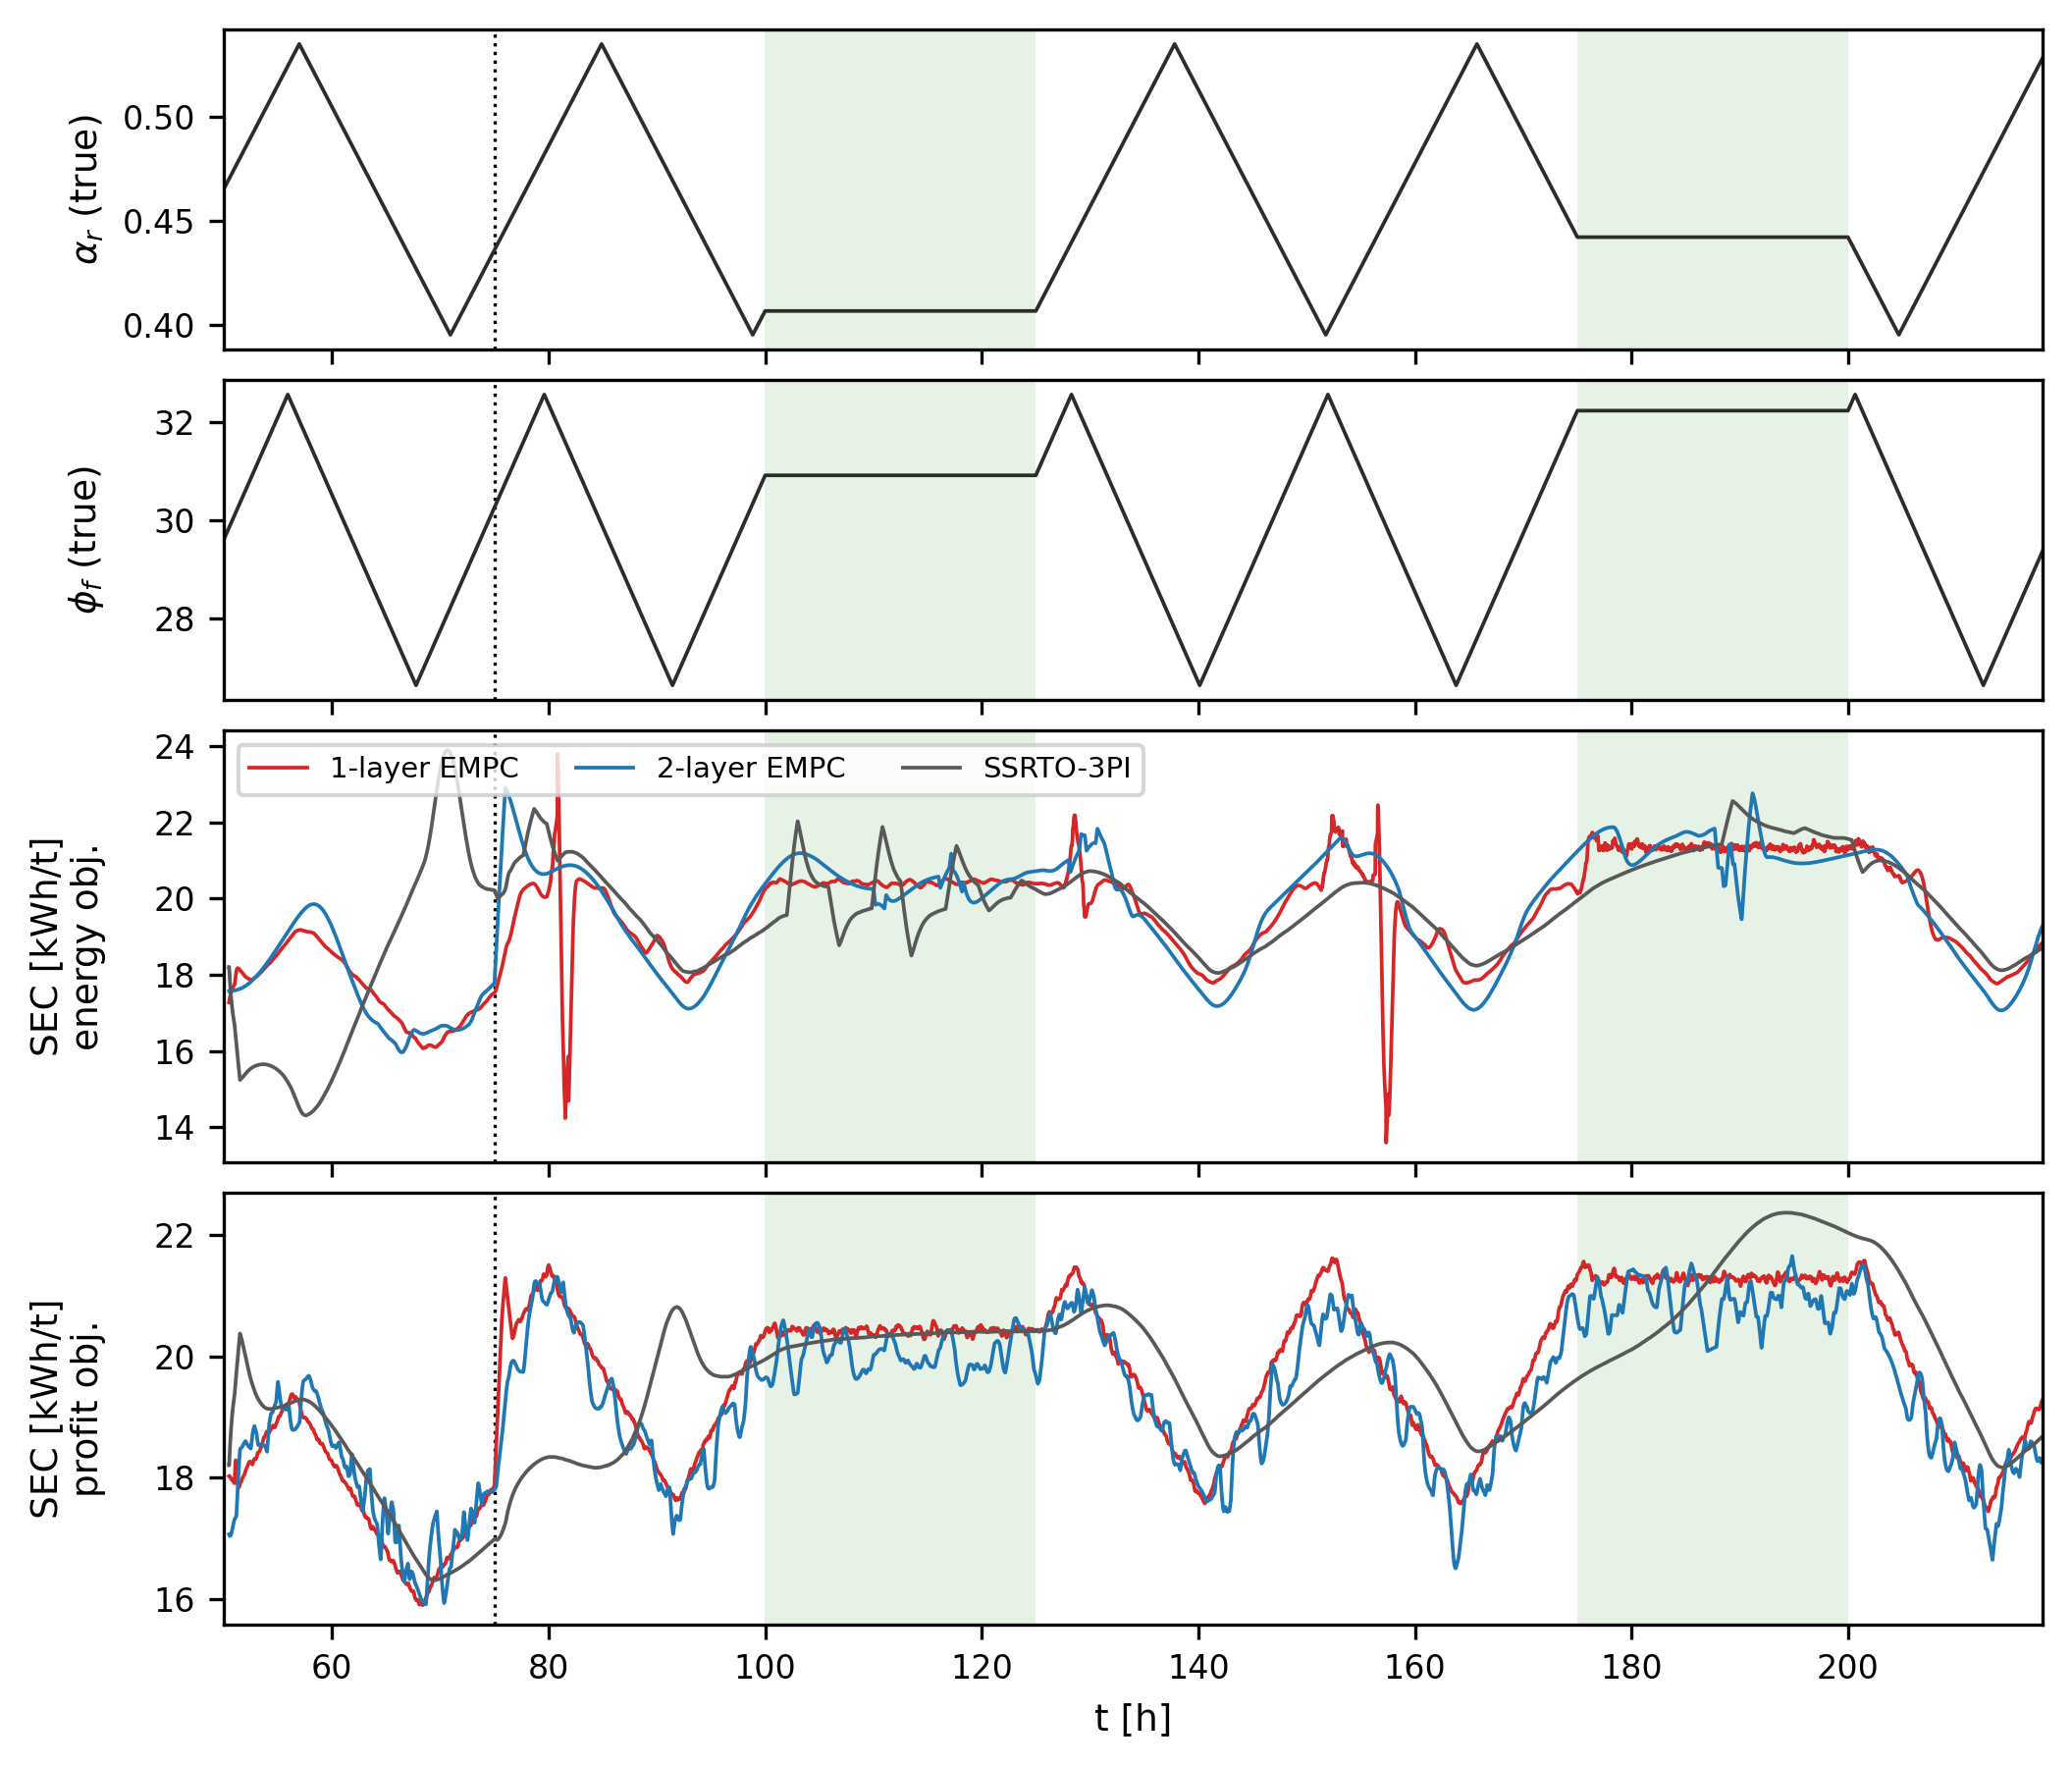
\includegraphics[width=\linewidth]{fig_ore_sec_time.png}
\caption{Top two panels: the v5 ore-hardness realisation (rock fraction
$\alpha_r$ and feed-size parameter $\phi_f$), identical in all six runs;
shaded bands are the ore holds, the dotted line the product-size floor
step. Bottom two panels: 1 h rolling specific energy of the three
architectures under the energy objective and the profit objective. SEC is
flat where the ore holds and varies where it ramps, for every architecture
and both objectives alike. The isolated spikes in the single-layer energy
trace are its occasional bang-bang episodes.}
\label{fig:oresec}
\end{figure}

\begin{figure}[t]
\centering
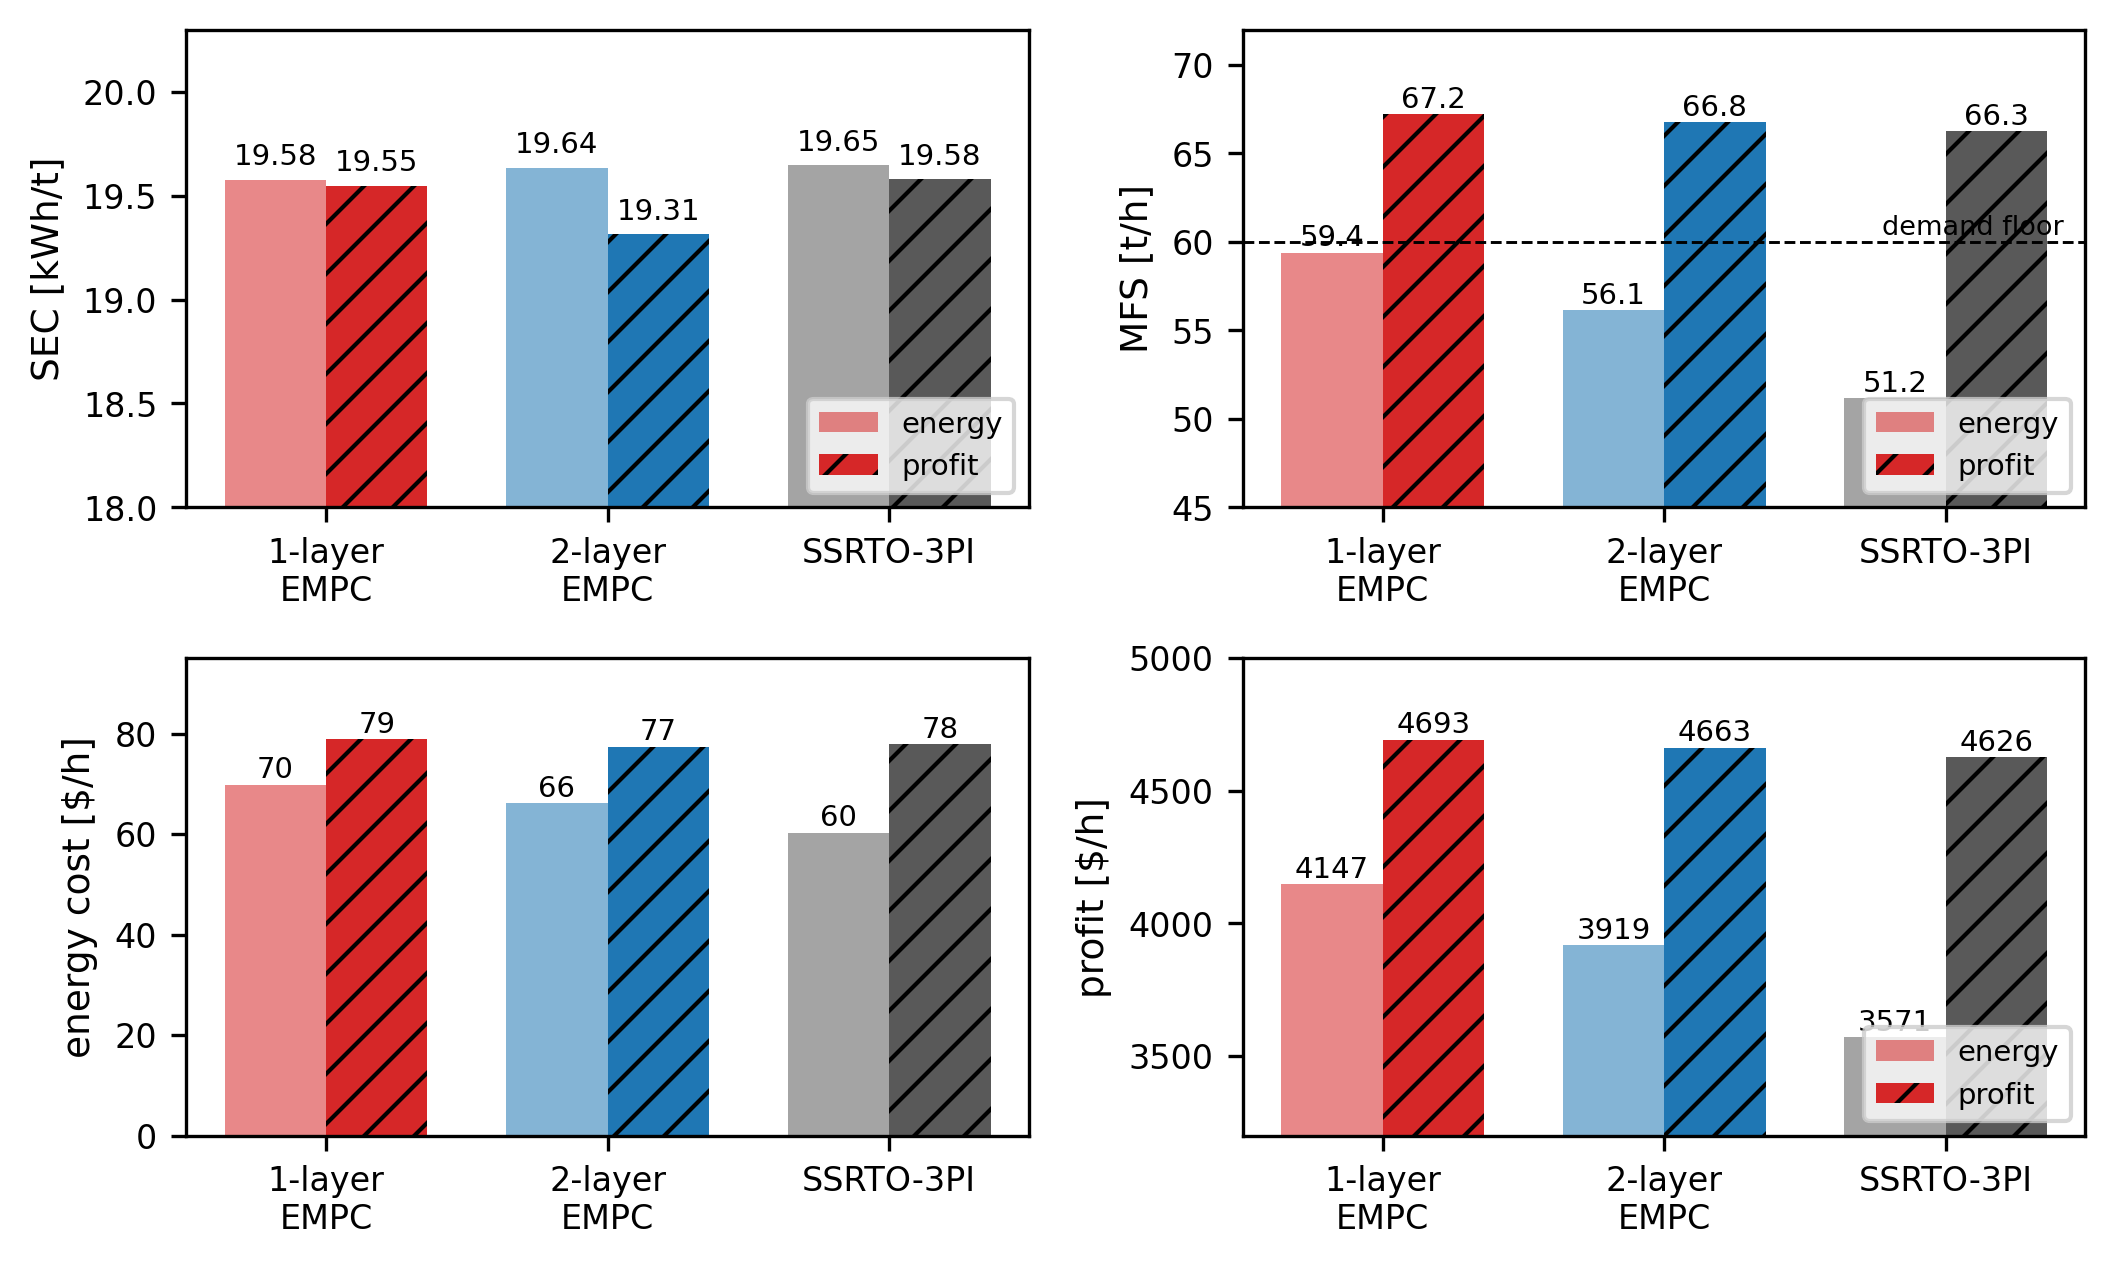
\includegraphics[width=\linewidth]{fig_sec_mfs_bars.png}
\caption{Run-average specific energy, feed rate, energy cost and profit
proxy for the three architectures under both objectives. SEC clusters
within about two percent across all six runs, while the operating points
differ. The profit objective lifts every architecture to 66--67 t/h, and
under the energy objective each architecture settles at a different feed
despite identical limits. The bottom row shows the economics. Energy cost
(60--79 \$/h) is under two percent of revenue in every run, which is why
the profit ranking is decided by tonnes.}
\label{fig:bars}
\end{figure}

\begin{table}[t]
\centering
\caption{Six matched-floor 218 h runs: specific energy, mean feed, energy
cost, and profit proxy ($A{=}71$ \$/t, $B{=}0.06$ \$/kWh), post-warm-up
window.}
\label{tab:summary}
\begin{tabular}{llrrrr}
\toprule
Architecture & Objective & SEC & MFS & Energy cost & Profit \\
 & & (kWh/t) & (t/h) & (\$/h) & (\$/h) \\
\midrule
1-layer EMPC & energy & 19.58 & 59.4 & 70 & 4147 \\
1-layer EMPC & profit & 19.55 & 67.2 & 79 & 4693 \\
2-layer EMPC & energy & 19.64 & 56.1 & 66 & 3919 \\
2-layer EMPC & profit & 19.31 & 66.8 & 77 & 4663 \\
SSRTO+3PI    & energy & 19.65 & 51.2 & 60 & 3571 \\
SSRTO+3PI    & profit & 19.58 & 66.3 & 78 & 4626 \\
\bottomrule
\end{tabular}
\end{table}

\subsection{The SEC cluster and its ore-hardness origin}

Table~\ref{tab:summary} and Fig.~\ref{fig:bars} give the central result.
At the matched product-size floor, the six runs span only 19.31 to 19.65
kWh/t. That is a spread of under two percent across three architectures
and two objectives. Fig.~\ref{fig:oresec} adds that the specific energy
of every run tracks the ore-hardness trajectory closely. SEC is flat
through the ore holds. It rises and falls with the feed-size parameter
through the ramps, with all three architectures moving together.

The model makes this connection explicit. Ore hardness enters the
reduced-order model as $\phi_f$, the power needed per tonne of new fines
produced inside the mill, in kWh/t \cite{leroux2013}. Specific energy is
its operational counterpart in the same unit.
$\mathrm{SEC}=P_{\mathrm{mill}}/\mathrm{MFS}$ is the energy spent per
tonne of fresh feed processed. Fines production is driven by mill power
through $\phi_f$. A pinned product-size floor fixes the fraction of each
feed tonne that must be ground to fines. SEC is therefore essentially a
scaled copy of $\phi_f$ (about 19.6 kWh/t against $\phi_f \approx 29.6$
kWh/t here, the ratio reflecting the fines already present in the feed).
The two quantities share one unit because they express the same
underlying physics, the energy the ore requires at the demanded fineness.
This is why every architecture returns nearly the same SEC under both
objectives, energy and profit (revenue minus energy), and why the SEC
trajectories in Fig.~\ref{fig:oresec} follow the ore-hardness
distribution so closely. Both objectives carry the energy term, and that
term is what pushes SEC to its achievable minimum. An objective without
an energy term would not settle at these values.

The controllers differ only in how well they avoid wasting energy
(over-grinding, poor set-point choices). None can grind below the energy
the ore demands. The distribution of achievable SEC is therefore a
property of the ore hardness distribution rather than of the supervisory
architecture or the economic objective.

One exception may apply to the SSRTO. Its set-points refresh only when
the steady-state detector triggers. If the ore hardness trends strongly
and rapidly in one direction without flattening, the detector cannot
trigger, and the SSRTO result can differ significantly. The disturbance
in Fig.~\ref{fig:oresec} instead fluctuates inside a bounded band of 10
to 15 percent.
The plant then keeps reaching steady states inside that band, and the
held set-points stay reasonable even when the detector does not
trigger. This can be why the SSRTO stays inside the two-percent cluster
here.

\subsection{Same limits, different operating points}

The clustering does not mean the architectures behave identically. Under
the energy objective the three architectures face the same feed-demand
floor, product-size floor and objective function. They still settle at
visibly different feeds of 59.4, 56.1 and 51.2 t/h for the single-layer,
two-layer and SSRTO respectively (Fig.~\ref{fig:bars}, right). Each
optimiser allocates the remaining degrees of freedom (mill speed, cyclone
feed, sump water) differently, and the SSRTO in particular drifts to
lower feed between its steady-state updates. Specific energy is the
invariant. The operating point is not. Under the profit objective the
picture collapses. All three lift feed to 66--67 t/h and mill speed to
its bound, confirming the constraint-seeking behaviour of Section~III-B.
The profit proxies land within 1.4 percent of one another (4626 to 4693
\$/h).

\subsection{Profit versus energy}

For each architecture the profit objective earns 13 to 29 percent more
profit proxy than its energy twin. Essentially all of the gain comes from
throughput. SEC changes by at most 0.33 kWh/t between the twins. The gain is largest
for the SSRTO only because its energy run sits at the lowest feed. In
other words, the profit objective adds tonnes by saturating feed and
speed limits, while its energy half holds SEC at the same level as the
energy runs. Which objective is appropriate therefore depends on whether
the mill is the right place to decide throughput, which is the subject
of the next section.

\subsection{Secondary separations}

The architectures do separate on non-economic metrics. The single-layer
EMPC shows occasional bang-bang episodes (isolated SEC spikes in
Fig.~\ref{fig:oresec}, roughly two percent of post-step intervals),
inherited from its near-affine objective. Because its set-point refreshes only
at steady-state detections, the SSRTO holds its product-size floor more
loosely than the EMPCs between updates. The PI loops themselves behave
exactly as designed. The two-layer EMPC shows neither behaviour and, as
noted in Section~IV, uses about a third less CPU time than the
single-layer. This combination, rather than any economic advantage, is
why we carry it forward as the main candidate.

\subsection{Comparison with the HPGR circuit study}

Our results are consistent with the HPGR, ball mill and flotation study
of Thivierge and co-authors \cite{thivierge2023}. They compared basic
regulatory control (BRC), advanced regulatory control (ARC), a profit
EMPC (EMPC1) and a power-penalised EMPC (EMPC2). Their ARC and EMPC1
performed identically because the economic optimum sits at the process
constraints. We see the same mechanism. Under the profit objective all
three of our architectures saturate feed and speed and land within 1.4
percent of one another. Their EMPC2 reduced specific energy by only 0.4
to 2.9 percent relative to the profit optimum, at the cost of 3.6 to
3.9 percent of net value. Our energy-versus-profit twins show the same
pattern (Section~VI-C). Finally, we excluded our own basic regulatory
variants, the tracking single-layer MPC and the decentralised 3PI, from
the benchmark (Section~IV). Those architectures used significantly more
energy, in line with their BRC result.

% =====================================================================
\section{Discussion}

\subsection{Plant-level profit, mill-level energy, and their interface}

The results give an operational answer to the objective question. Profit
optimisation is the natural plant-wide objective. Only at that level do
the downstream circuits (flotation recovery, concentrate value, market
prices) enter, and only there does Eq.~(\ref{eq:jcomm}) have its interior
optimum. At the SAG level the same objective reduces to feed-and-speed
saturation, a standing choice that removes every degree of freedom that
could otherwise be used for efficiency or robustness. Energy
minimisation, by contrast, is well posed at the mill. It has a defined
task, to grind the demanded tonnes to the demanded fineness for the least
energy. As Section~VI shows, it concedes nothing in specific energy
relative to the profit objective.

Once quality is pinned, the achievable specific energy is set by the
ore. The remaining economic decision is how many tonnes to process.
That decision belongs to the plant-wide layer. The two levels meet at a
two-number interface. It consists of a
throughput demand $\mathrm{TP}_{\mathrm{dem}}$ (a floor on MFS) and a
product-size floor $\mathrm{PSE}_{\min}$. The plant-wide profit
optimisation, which sees all circuits, decides the most profitable
throughput and hands it down. The downstream circuits' requirements set
the product-size floor. Inside those limits the mill runs autonomously
and never needs to maximise MFS directly. The demand floor already
encodes how many tonnes the plant wants. The controller contains no
downstream model, no prices and no ore body assumptions, so it ports
across plants unchanged. Re-targeting it is a change of two numbers
rather than a re-identification.

The interface also carries a safety and flexibility argument. Because the
mill works around the lower and safer limits rather than pushing to a
maximum, the operator or the
plant-wide layer can derate it through the same knobs, for example
capping MFS during downstream maintenance or an electrical demand event.
The controller then simply optimises energy inside the tighter envelope.
A profit-maximising mill instead works at full speed. The mill speed
$\phi_c$ reaches its maximum and stays there, which is not a safe
condition for continuous operation.

\subsection{Two-layer EMPC as the practical embodiment}

The two-layer EMPC splits the mill controller itself into two
timescales. The slow upper layer solves the economic problem inside the
interface limits. The fast lower layer tracks it. Our benchmark indicates
this costs nothing measurable in specific energy relative to the
single-layer ideal. It removes the bang-bang failure mode, reduces
computation by about a third, and retains transient responsiveness that
the classical SSRTO reference lacks. The SSRTO remains attractive for its
negligible computational cost, and its economics are within two percent
here. Its loose quality tracking between steady-state updates, however,
makes it the weakest of the three at holding the interface contract that
the modular separation depends on.

% =====================================================================
\section{Conclusion}

On a single-stage SAG circuit with identical ore, estimator and
constraints, we benchmarked three supervisory architectures under both
candidate economic objectives. Two findings stand out.

The first is the SEC similarity. Once every requirement is made
identical, the specific energy of all six combinations converges to
within about two percent and follows the ore-hardness disturbance. With
a well-chosen optimisation, energy minimisation or a profit objective
that includes the energy term, the controller reaches the achievable
SEC. That achievable SEC is directly correlated with the ore hardness.
None of the controllers can grind below the energy the ore demands. The
distribution of achievable SEC is therefore a property of the ore
hardness distribution rather than of the supervisory architecture or the
economic objective. Most published comparisons cannot observe this
because each controller is evaluated with its own model, estimator,
constraint set and tuning. The architectures still choose different
operating points under identical limits, so the equivalence is in energy
per tonne, not in behaviour.

The second is the choice between profit and energy optimisation. Profit
maximisation does two things at once. It maximises throughput and
minimises energy, which is why it too reaches the achievable SEC.
Maximising throughput can be a good choice in some cases, for example
when the mill is the plant bottleneck. In general it is bad practice. It
holds feed and mill speed at their limits continuously. Liner and media
wear grow steeply with speed, liner changes are long downtime events,
and high speed at low charge throws balls directly onto the liners.
Energy minimisation is the better objective for the SAG circuit. It also
makes the mill completely modular. Once profit optimisation is removed,
the SAG mill becomes independent of the other circuits and of the plant.
Through the MFS and PSE interface it can be integrated into any plant
and any circuit. A heat map of MFS, PSE and SEC, where SEC represents
the ore hardness, defines the best working regions. Such maps summarise
the dynamic model and can be used in complex plant-wide calculations.

This suggests a direction for real-time optimisation practice. At the
plant-wide level, economic calculations run together with planning and
scheduling information, and steady-state calculations are the practical
choice. At the circuit level, transient operation can be exploited
through EMPC with an objective consistent with the plant objective.
Forcing the same states and the same optimisation onto both levels can
be bad practice. It is worth remembering that the classic SSRTO applies
the steady-state assumption at both levels and waits too long for the
plant to settle.

This study is an early stage of an ongoing research program. We kept
its scope deliberately small so that the comparison stayed clean. All
runs use one synthetic ore realisation, a single 218 h protocol, and
fixed plant and economic parameters. Only the two ore hardness
parameters vary. Slowly varying effects such as liner wear are left
for future work. Efforts to obtain representative plant data are
ongoing. The next steps are to calibrate the model against historical
operating data and to run longer, more varied scenarios so the
architectures can be separated with statistical confidence.

\section*{Acknowledgment}

This work is supported by a Curtin University research scholarship.

\begin{thebibliography}{00}
\bibitem{leroux2013} J. D. le Roux, I. K. Craig, D. G. Hulbert, and A. L.
Hinde, ``Analysis and validation of a run-of-mine ore grinding mill
circuit model for process control,'' \emph{Minerals Engineering}, vol.
43--44, pp. 121--134, 2013.
\bibitem{leroux2019} J. D. le Roux and I. K. Craig, ``Plant-wide control
framework for a grinding mill circuit,'' \emph{Industrial and Engineering
Chemistry Research}, vol. 58, pp. 11585--11600, 2019.
\bibitem{thivierge2023} A. Thivierge, J. Bouchard, and A. Desbiens,
``Comparing economic model predictive control to basic and advanced
regulatory control on a simulated HPGR, ball mill, and flotation
circuit,'' \emph{Journal of Process Control}, vol. 122, pp. 159--171,
2023.
\bibitem{leroux2022} J. D. le Roux and C. W. Steyn, ``Validation of a
dynamic non-linear grinding circuit model for process control,''
\emph{Minerals Engineering}, vol. 187, p. 107780, 2022.
\bibitem{leroux2017} J. D. le Roux, A. Steinboeck, A. Kugi, and I. K.
Craig, ``An extended Kalman filter observer to estimate the hold-ups of a
semi-autogenous grinding mill,'' \emph{Journal of Process Control}, vol.
51, pp. 27--41, 2017.
\bibitem{matias2022} J. Matias, J. P. C. Oliveira, J. D. le Roux, and J.
J\"{a}schke, ``Steady-state real-time optimization using transient
measurements,'' \emph{Journal of Process Control}, vol. 115, pp. 181--196,
2022.
\bibitem{ellis2017} M. Ellis, J. Liu, and P. D. Christofides,
\emph{Economic Model Predictive Control: Theory, Formulations and Chemical
Process Applications}. Springer, 2017.
\end{thebibliography}

\end{document}
